\section{Taking Control}
\label{sec:taking_control}

\subsection{Variables}
\label{sub:variables}
\begin{frame}[fragile]
	\frametitle{Variables}
	A variable is a container that has:
	\begin{description}
		\item [Type] What data it can hold
		\item [Identifier] The name you access it with
		\item [Value] The data it holds
		\item [Scope] Where you can access it from
	\end{description}
	\vfill
	You must declare a variable before you can use it:
	\begin{lstlisting}[numbers=none]
		type identifier = value;
	\end{lstlisting}
	The value is optional if you do not need a starting value.
\end{frame}

\begin{frame}
	\frametitle{Variable Types}
	\begin{tabular}{r|c|c|l}
		Format & Type & Bits & Range\\
		\hline
		Integer & char & 8 & 0 -- 255\\
		& signed char & 8 & -128 -- 127\\
		& unsigned short & 16 & 0 -- 65,535\\
		& short & 16 & -32,768 -- 32,767\\
		& unsigned int & 32 & 0 -- 4,294,967,295\\
		& int & 32 & $2.1 \times 10^9$ -- $2.1 \times 10^9$\\
		& unsigned long long & 64 & 0 -- $1.8 \times 10^{19}$\\
		& long long & 64 & $-9 \times 10^{18}$ -- $9 \times 10^{18}$\\
		\hline
		Floating & float & 32 & $-3.4 \times 10^{38}$ -- $3.4 \times 10^{38}$\\
		& double & 64 & $-1.7 \times 10^{308}$ -- $1.7 \times 10^{308}$\\
	\end{tabular}
	\begin{block}{Note}
		The mbed natively works with 32 bit types, a huge advantage over 8 and 16 bit processors
	\end{block}
\end{frame}

\begin{frame}[fragile]
	\frametitle{Variable Scope}
	Variable scope is set by where a variable is declared:
	\begin{columns}[c]
		\begin{column}{0.5\textwidth}
			\begin{lstlisting}[numbers=none]
				int a = 0;
				
				int main() {
				  float b = 0.0f;
				  while(true) {
				    double c = 0.0;
				  }
				}
			\end{lstlisting}
		\end{column}
		\begin{column}{0.5\textwidth}
			\begin{itemize}
				\item a is outside any functions and can be seen anywhere in the file
				\item b can be seen anywhere inside main()
				\item c can only be seen inside the while loop
			\end{itemize}
		\end{column}
	\end{columns}
	A simple rule of thumb is a variable can only be seen inside its enclosing braces.
	\begin{block}{Best Practice}
		Use the narrowest scope possible
	\end{block}
\end{frame}

\begin{frame}
	\frametitle{Using Variables}
	\begin{columns}[c]
		\begin{column}{0.5\textwidth}
			\begin{center}
				\begin{tabular}{c|l}
					\multicolumn{2}{c}{Arithmetic Operators}\\
					\hline
					= & assignment\\
					+ & addition\\
					- & subtraction\\
					* & multiplication\\
					/ & division\\
					\% & modulus\\
				\end{tabular}
				\vfill
				\begin{tabular}{c|l}
					\multicolumn{2}{c}{Bitwise Operators}\\
					\hline
					\& & bitwise and\\
					| & bitwise or\\
					\^{} & bitwise xor\\
					\~{} & bitwise not\\
					<< & bitshift left\\
					>> & bitshift right\\
				\end{tabular}
			\end{center}
		\end{column}
		\begin{column}{0.5\textwidth}
			\begin{center}
				\begin{tabular}{c|l}
					\multicolumn{2}{c}{Compound Operators}\\
					\hline
					++ & increment\\
					-{-} & decrement\\
					+= & compound addition\\
					-= & compound subtraction\\
					*= & compound multiplication\\
					/= & compound division\\
					\&= & compound bitwise and\\
					|= & compound bitwise or\\
				\end{tabular}
			\end{center}
		\end{column}
	\end{columns}
\end{frame}

\subsection{Digital Input}
\label{sub:digital_input}
\begin{frame}[fragile]
	\frametitle{Digital Input}
	\begin{lstlisting}[numbers=none]
		DigitalIn(PinName pin, PinMode mode);
	\end{lstlisting}
	DigitalIn operates nearly identically to DigitalOut, except you can optionally specify a pin mode:
	\begin{description}
		\item[PullNone] Standard mode, default
		\item[PullUp] Weak pull up resistor enabled
		\item[PullDown] Weak pull down resistor enabled
	\end{description}
	Access the value of the pin by treating it like any other variable.
	\begin{block}{Example}
		\begin{lstlisting}[numbers=none]
			DigitalIn btn(USER_BUTTON);
			int state = btn;
		\end{lstlisting}
	\end{block}
\end{frame}

\begin{frame}[fragile]
	\frametitle{A New Program}
	\begin{columns}[T]
		\begin{column}{0.5\textwidth}
			Create a new program with:
			\begin{itemize}
				\item DigitalIn on the button
				\item DigitalOut on the LED
				\item Infinite main loop
				\item Button controlling the LED
			\end{itemize}
			\begin{block}{Tip}
				Look at the pin diagrams to determine what PinName to use
			\end{block}
		\end{column}
		\begin{column}{0.5\textwidth}
			\pause
			\lstinputlisting[title=TakingControl.cpp]{code/taking_control/1.cpp}
		\end{column}
	\end{columns}
\end{frame}

\subsection{Conditional Statements}
\label{sub:conditional_statements}
\begin{frame}
	\frametitle{Conditional Statements}
	Conditional statements are constructed from comparison and boolean operators:
	\begin{columns}[T]
		\begin{column}{0.5\textwidth}
			\begin{center}
				\begin{tabular}{c|l}
					\multicolumn{2}{c}{Comparison Operators}\\
					\hline
					== & equal to\\
					!= & not equal to\\
					< & less than\\
					> & greater than\\
					<= & less than or equal to\\
					>= & greater than or equal to\\
				\end{tabular}
			\end{center}
		\end{column}
		\begin{column}{0.5\textwidth}
			\begin{center}
				\begin{tabular}{c|l}
					\multicolumn{2}{c}{Boolean Operators}\\
					\hline
					\&\& & and\\
					|| & or\\
					! & not\\
				\end{tabular}
			\end{center}
		\end{column}
	\end{columns}
\end{frame}

\begin{frame}[fragile]
	\frametitle{If Statements}
	An if statement executes different code based on the result of a conditional statement:
	\begin{lstlisting}[numbers=none]
		if(x > 0) {
		  // Run if x is positive
		} else if(x < 0) {
		  // Run if x is negative
		} else {
		  // Run otherwise
		}
	\end{lstlisting}
	The else if and else clauses are optional. For simple cases, so are the braces:
	\begin{lstlisting}[numbers=none]
		if(x < 0) x = 0;
	\end{lstlisting}
\end{frame}

\begin{frame}[fragile]
	\frametitle{Revisiting Our Last Program}
	Try to rewrite the last program using an if statement instead of simple assignment
	\pause
	\lstinputlisting[title=TakingControl.cpp]{code/taking_control/2.cpp}
\end{frame}

\begin{frame}
	\frametitle{A Note on Logic Levels}
	A common practice is to use a pull-up resistor on buttons:
	\begin{columns}[c]
		\begin{column}{0.5\textwidth}
			\begin{itemize}
				\item Forces a known logic state
				\item \textbf{Inverts logic levels!}
				\item You can do this yourself using the PinMode parameter of DigitalIn objects
			\end{itemize}
		\end{column}
		\begin{column}{0.5\textwidth}
			\begin{center}
				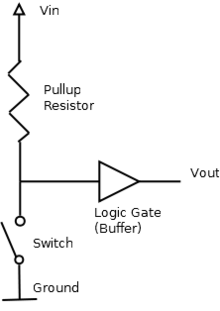
\includegraphics[height=0.5\paperheight]{pullup}\\
			\end{center}
		\end{column}
	\end{columns}
	\ccbysa{http://commons.wikimedia.org/wiki/File:Pullup_Resistor.png}{C4VC3}
\end{frame}

\subsection{A Better Blinker}
\label{sub:better_blink}
\begin{frame}
	\frametitle{A Better Blinker}
	Lets try rewriting the blinky LED program to be a little more useful: use the button to change the delay time
	\pause
	\begin{itemize}
		\item Use a global variable to count button presses
		\item Remember the button has inverted logic levels
		\item Check the bounds of your count
		\item Try using math instead of discrete states
	\end{itemize}
\end{frame}

\begin{frame}[fragile]
	\frametitle{One Solution}
	\lstinputlisting[title=BetterBlink.cpp,multicols=2]{code/taking_control/3.cpp}
\end{frame}

\begin{frame}[fragile]
	\frametitle{A More Elegant Solution}
	\lstinputlisting[title=BetterBlink.cpp]{code/taking_control/4.cpp}
\end{frame}